\documentclass{standalone}
\usepackage{tkz-base}
\usepackage{tkz-fct}
\usepackage{tkz-euclide}
\usepackage{tikz}
\begin{document}
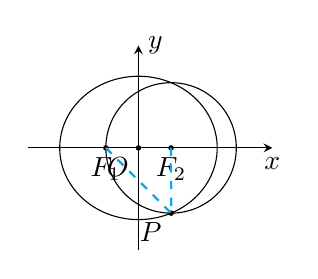
\begin{tikzpicture}
\pgfmathsetmacro\x{1.4}
\pgfmathsetmacro\y{1.3}
\pgfmathsetmacro\a{1}
\pgfmathsetmacro\c{sqrt(2)-1}
\pgfmathsetmacro\b{sqrt(abs(\a^2-\c^2))}
\coordinate (O) at (0,0);
\coordinate (F1) at (-\c,0);
\coordinate (F2) at (\c,0);
\draw[-stealth] (-\x,0) -- (\x+0.3,0) node [below] {$x$};
\draw[-stealth] (0,-\y) -- (0,\y) node [right] {$y$};
\draw[name path = a ] (F2) circle (2*\c);
\draw[name path = b ] (O) circle [x radius=\a,y radius=\b];
\fill [name intersections={of=a and b,by={Q,P}}](P) circle (1pt) node [below left] {$P$};
\fill (O) node [below left] {$O$} circle (1pt);
\fill (F1) node [below] {$F_1$} circle (1pt);
\fill (F2) node [below] {$F_2$} circle (1pt);
\draw[cyan,dashed,thick] (F1) -- (P)-- (F2);
 \end{tikzpicture}
\end{document}